\documentclass[hyperref={pdfpagelabels=false}]{beamer}

\usetheme{Heidelberg}

\usepackage{wrapfig}
\usepackage{lmodern}
\usepackage{natbib}
\usepackage{amsmath,amsfonts,amssymb}
\usepackage{algorithm,algorithmic}

\usepackage{natbib}

%\usepackage{tikz}
%	\usetikzlibrary[topaths,arrows,calc]
%\usepackage{wrapfig}
\usepackage{graphicx}
%\usepackage{stackengine}
\usepackage{subcaption}
\captionsetup[subfigure]{labelformat=empty}


\usepackage[english]{babel}
\usepackage[T1]{fontenc} % Ligaturen, richtige Umlaute im PDF 
\usepackage[utf8]{inputenc}% UTF8-Kodierung für Umlaute usw

\usepackage{hyperref}

\definecolor{darkred}{rgb}{110,1,1}  
\definecolor{maroon}{rgb}{0.5,0,0}  

\newcounter{saveenumi}
\newcommand{\seti}{\setcounter{saveenumi}{\value{enumi}}}
\newcommand{\conti}{\setcounter{enumi}{\value{saveenumi}}}


% zusaetzlich ist das usepackage{beamerthemeshadow} eingebunden 
\usepackage{beamerthemeshadow}

\renewcommand{\thefootnote}{\fnsymbol{footnote}} 

%--------------------------------------------------------------------------%
%--------------------------------------------------------------------------%
\def\vec{\mathop{\rm vec}}								% matrix vectorization
\def\tr{\mathop{\rm tr}}								% matrix trace
\def\argmax{\mathop{\rm argmax}}						% argmax
\def\argmin{\mathop{\rm argmin}}						% argmin
\def\median{\mathop{\rm median}} 						% median
\def\dist{\mathop{\rm dist}} 						    % dist
%--------------------------------------------------------------------------%
%--------------------------------------------------------------------------%
\title[Application of graph matching in Computer Vision]
	{Application of graph matching in Computer Vision}
\subtitle{Master Seminar}
\author[E.~Tikhoncheva] % (optional, for multiple authors)
	{Ekaterina~Tikhoncheva}
\institute[Universities Here and There] % (optional)
	{University of Heidelberg\\
	Faculty of Mathematics and Computer Science \\
	Computer Vision group \\
	at\\
	Heidelberg Collaboratory for Image Processing
}
\date[2015]{November 2015}
%--------------------------------------------------------------------------%
%--------------------------------------------------------------------------%
%--------------------------------------------------------------------------%
\begin{document}
\begin{frame}
\titlepage
\end{frame}
%--------------------------------------------------------------------------%
\begin{frame}
\frametitle{Agenda}
\tableofcontents
\end{frame} 
%--------------------------------------------------------------------------%
%--------------------------------------------------------------------------%
\section{Graph matching} 
\subsection{Introduction}
\begin{frame}[allowframebreaks]
\frametitle{Attributed undirected graph}

Attributed undirected graph $G=(V,$
\begin{itemize}
\item set of nodes $V=\{v_i\}_{i=1}^{n}$
\end{itemize}
\vspace{2cm}
\begin{figure}[b]
    \centering
    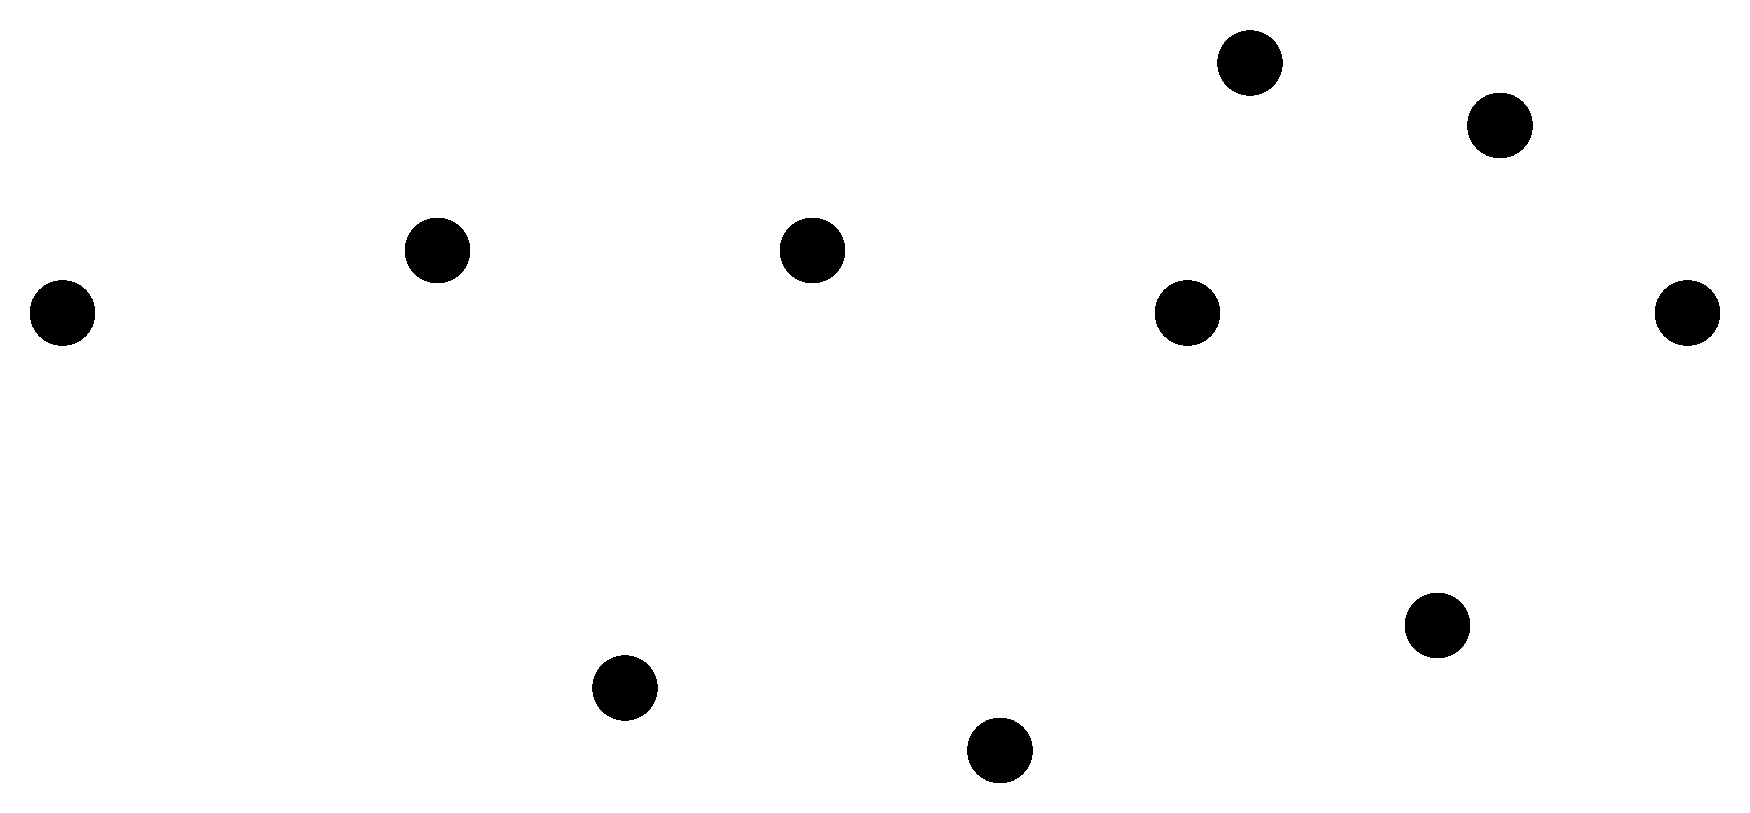
\includegraphics[width=5cm]{fig/graph_1_nodes.pdf}
\end{figure}%
%\end{frame}
\framebreak
%--------------------------------------------------------------------------%
%\begin{frame}
\frametitle{Attributed undirected graph}
Attributed undirected graph $G=(V,E,$
\begin{itemize}
\item set of nodes $V=\{v_i\}_{i=1}^{n}$
\item set of edges $E\subseteq\{\{u,v\}| u, v\in V\}$
\end{itemize}
\vspace{1.5cm}
\begin{figure}[b]
    \centering
    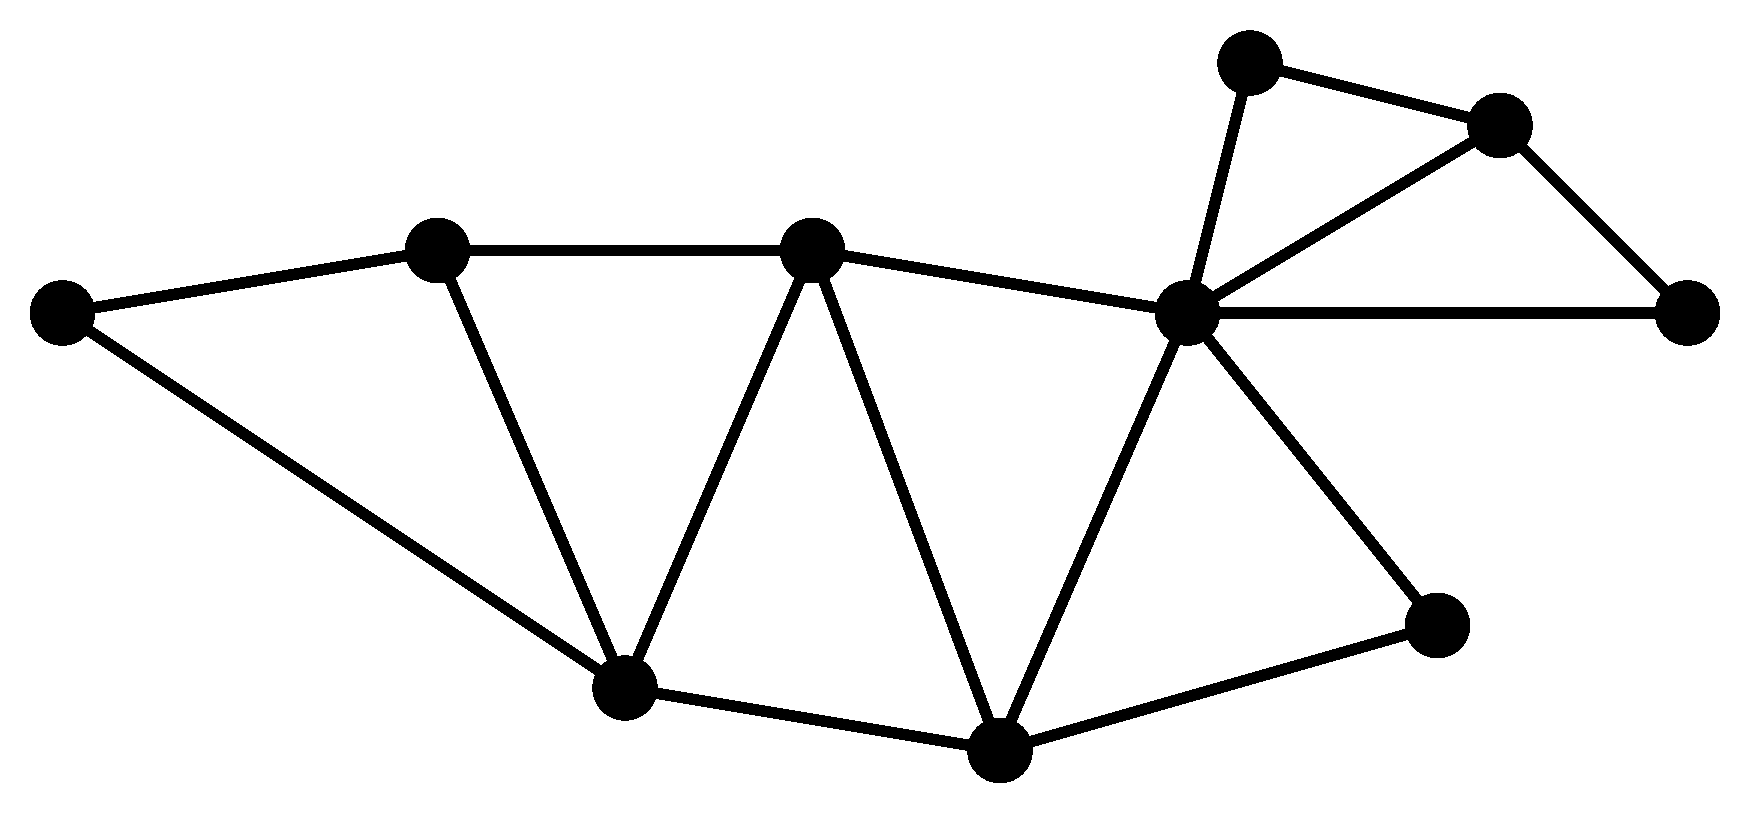
\includegraphics[width=5cm]{fig/graph_1.pdf}
\end{figure}%
\end{frame}
%--------------------------------------------------------------------------%
\begin{frame}
\frametitle{Attributed undirected graph}
Attributed undirected graph $G=(V,E,D)$
\begin{itemize}
\item set of nodes $V=\{v_i\}_{i=1}^{n}$
\item set of edges $E\subseteq\{\{u,v\}| u, v\in V\}$
\item node attributes $D=\{d_i\}_{i=1}^{n}$, $D\subset\mathbb{R}^r$
\end{itemize}
\vspace{1cm}
\begin{figure}[b]
    \centering
    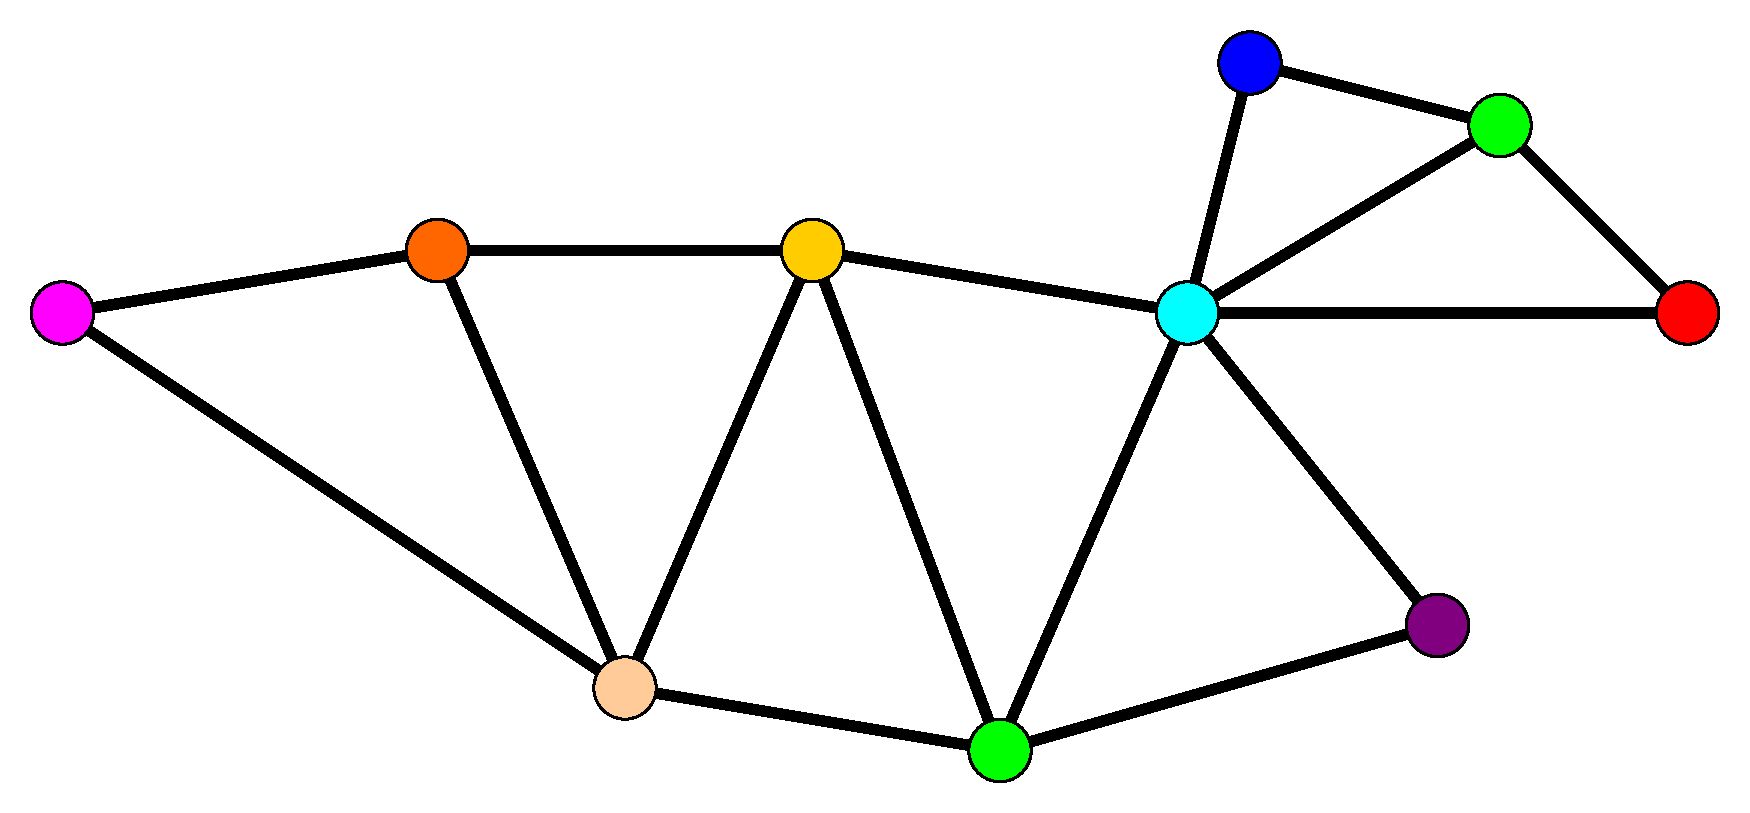
\includegraphics[width=5cm]{fig/at_graph_1.pdf}
\end{figure}%
\end{frame}
%--------------------------------------------------------------------------%
\subsection{Graph matching}
\begin{frame}
\frametitle{Graph matching}
Let us consider two undirected attributed graphs $G^I = (V^I, E^I, D^I)$ and $G^J = (V^J, E^J,D^J)$: % with $|V^I|=n_1$ and $|V^J|=n_2$:
\begin{figure}[h]
        \centering
        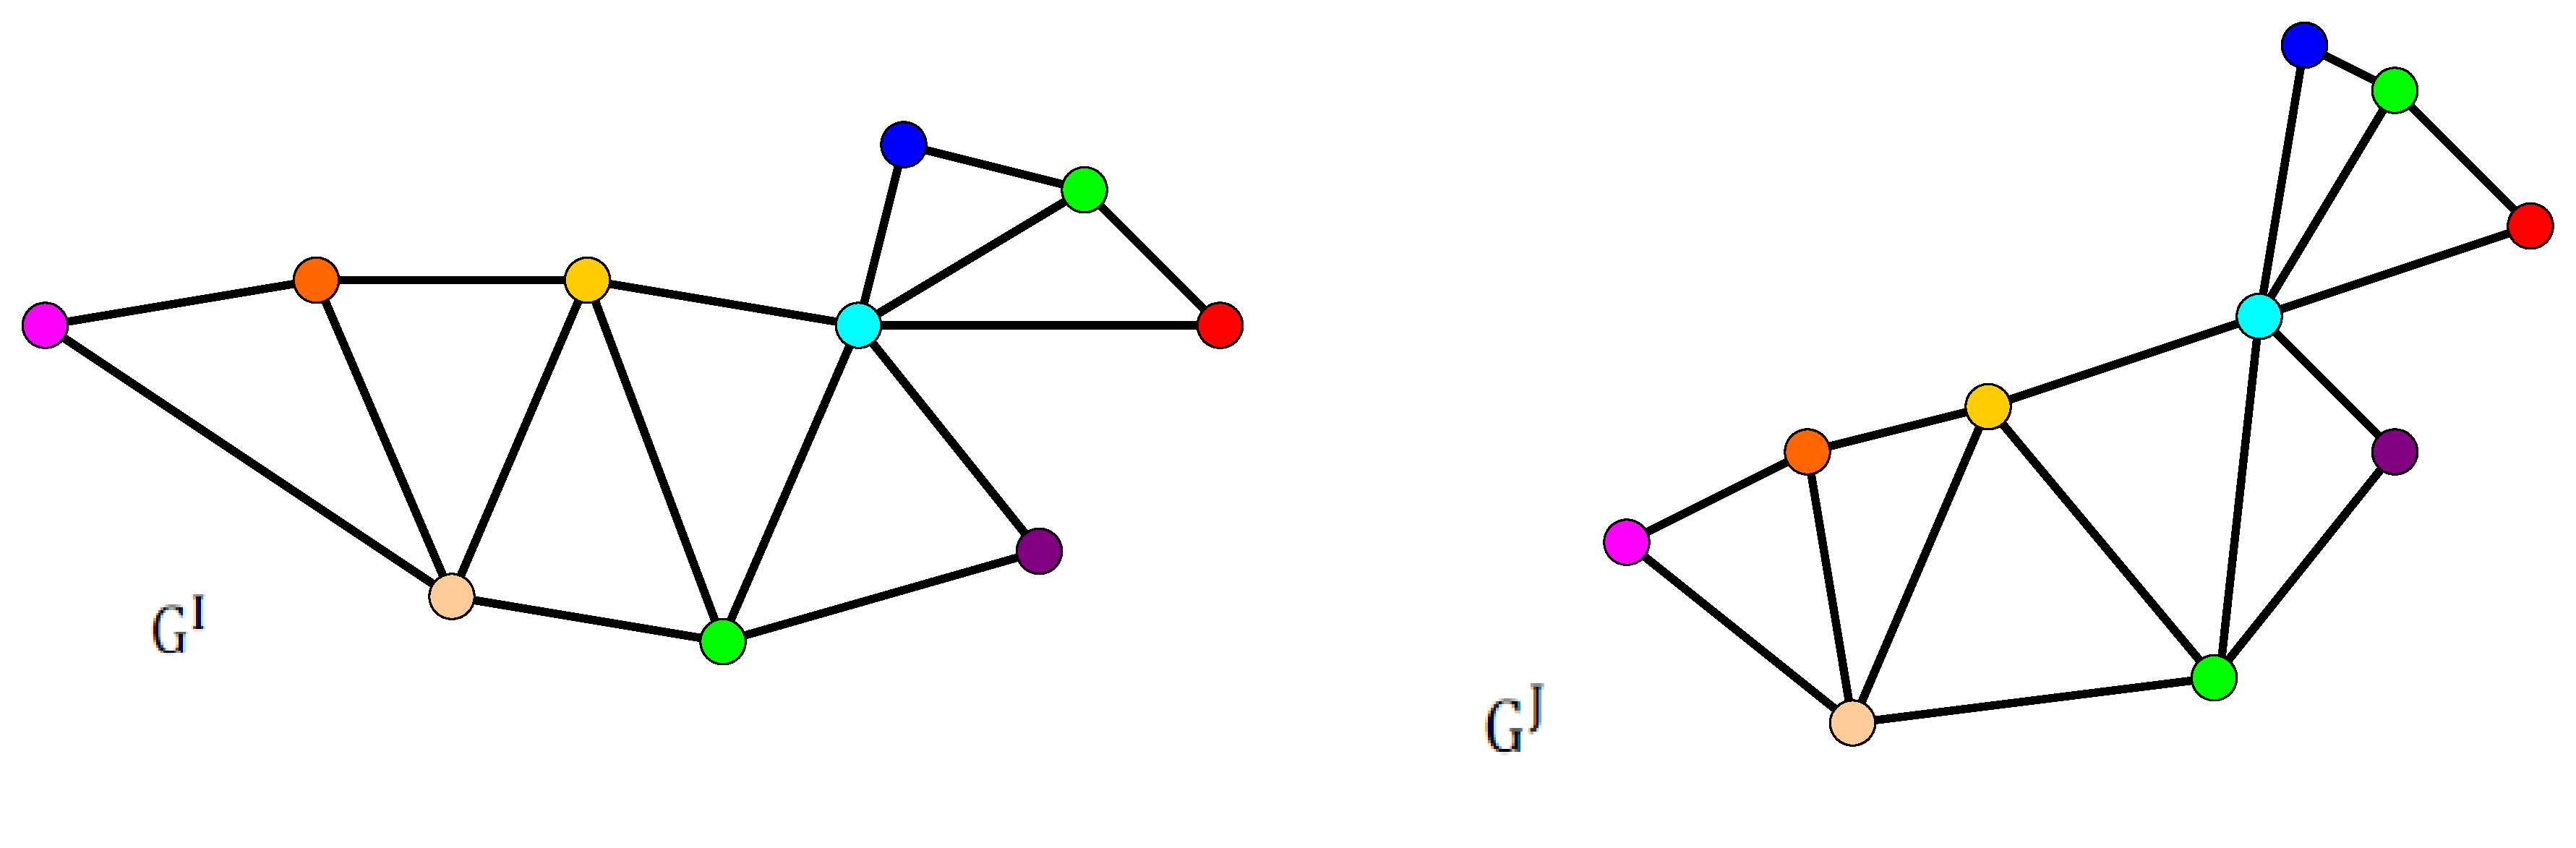
\includegraphics[width=6cm]{fig/graphs_12.pdf}
\end{figure}
%A matching function between $G^I$ and $G^J$ is a mapping $m:V^I\rightarrow V^J$ between the sets of nodes of two graphs.
\end{frame}
%\framebreak
%--------------------------------------------------------------------------%
\begin{frame}
\frametitle{Graph matching}
\begin{figure}[t]
        \centering
        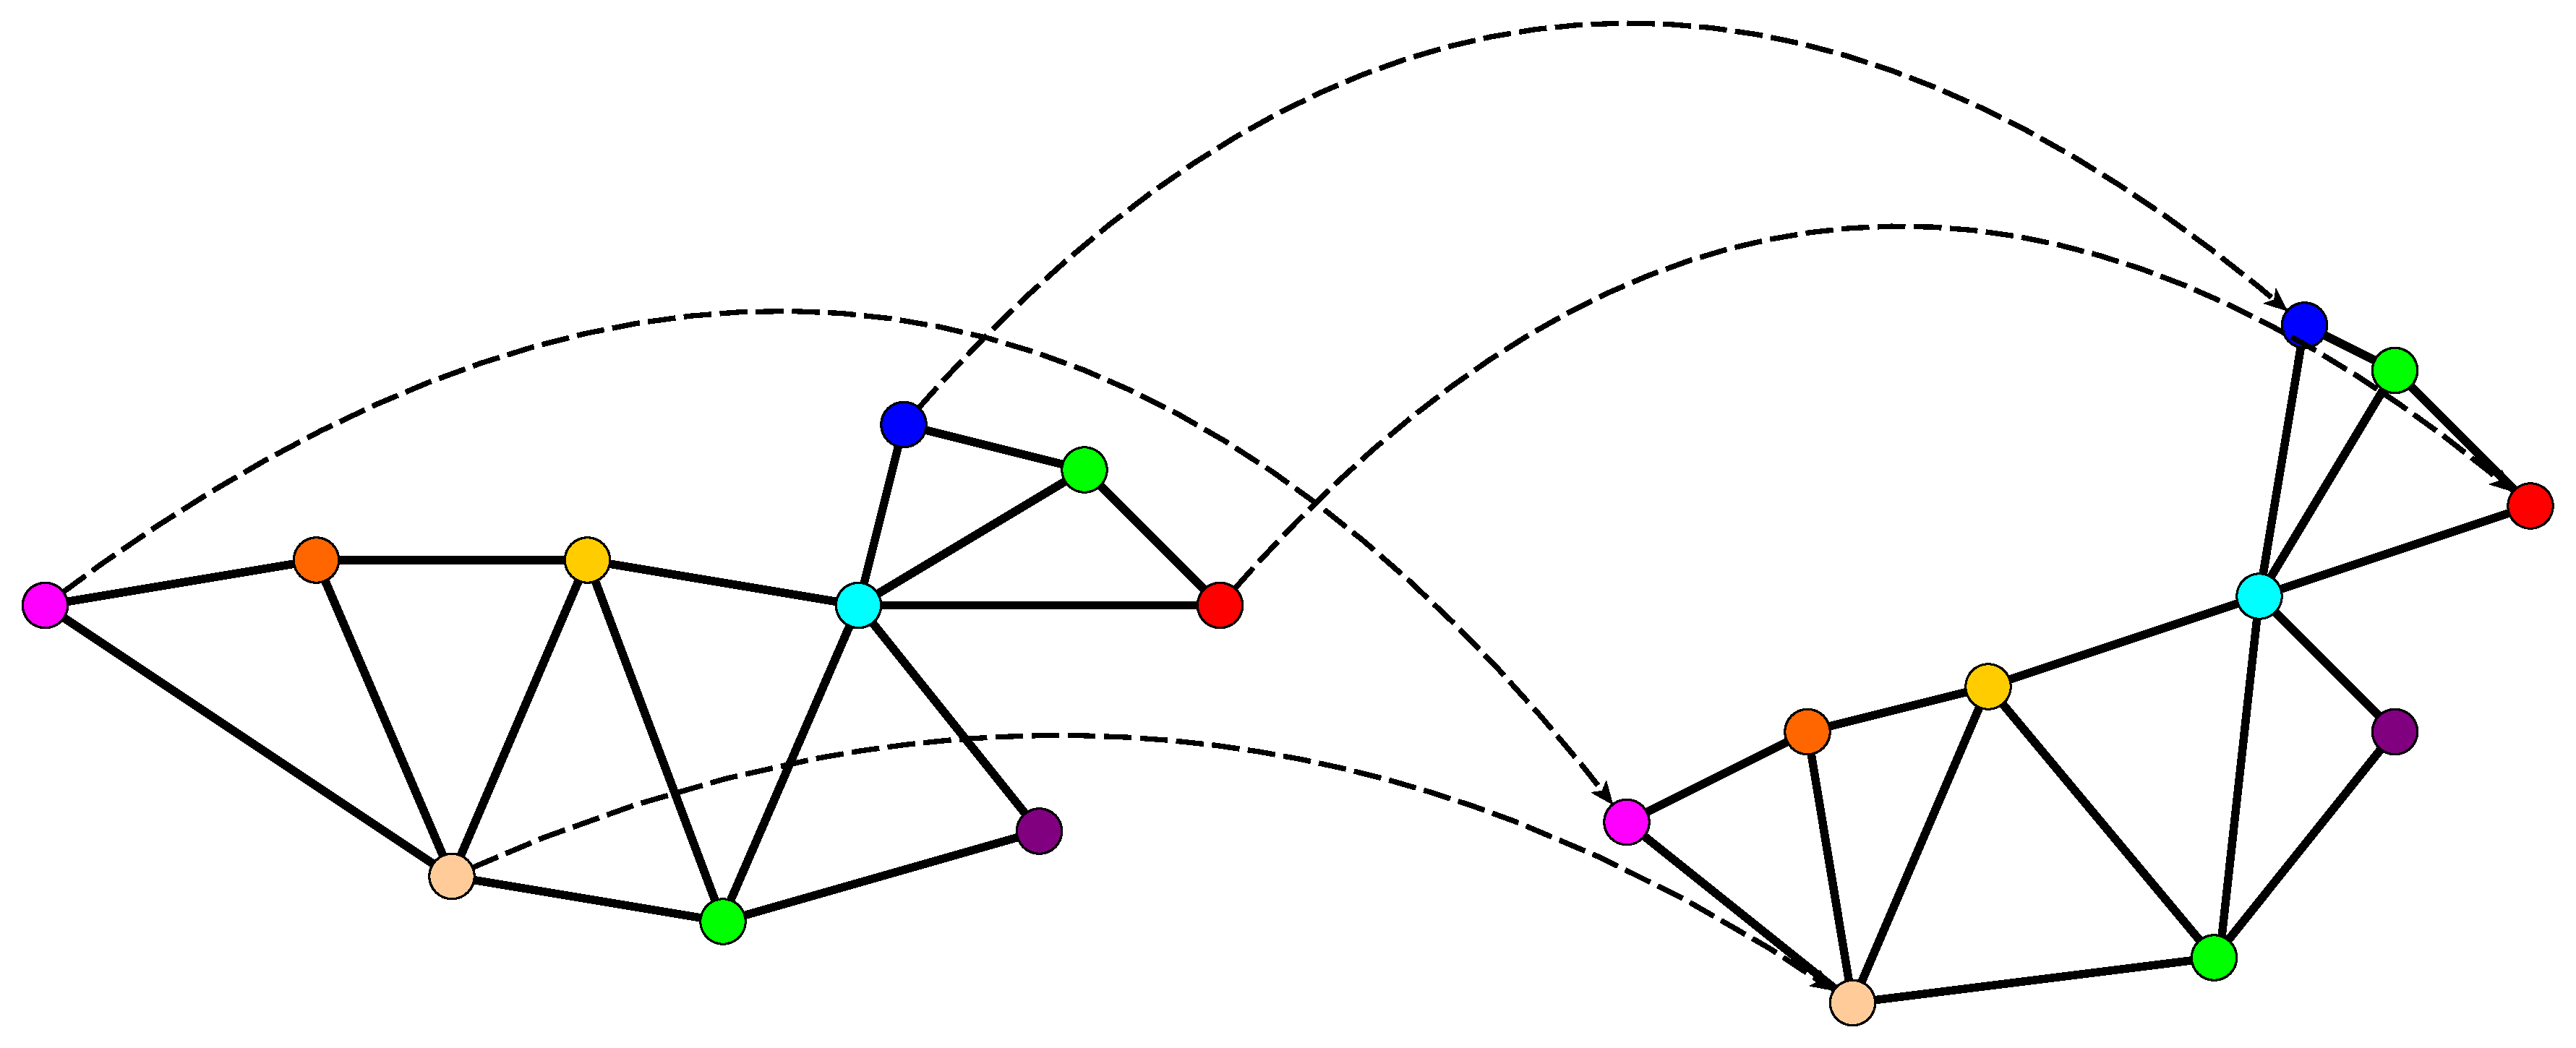
\includegraphics[width=5cm]{fig/matching_12.pdf}
\end{figure}
A matching function between $G^I$ and $G^J$ is a mapping %between the sets of nodes of two graphs:
\\
{\hspace{4cm}$m:V^I\rightarrow V^J$}
\visible<2>{\textcolor{red}{\hspace{2cm}not unique!}}
\visible<3->{
Define a function $S(G^I, G^J, m)$ to measure the quality of matching $m$ that fulfills some constraints\\
$\Rightarrow$ \textcolor{red}{Graph matching problem} between $G^I$ and $G^J$ 
\begin{equation*}
m = \argmax_{\hat{m}}S(G^I, G^J, \hat{m})
\end{equation*}
}
\end{frame}
%--------------------------------------------------------------------------%
\begin{frame}
\frametitle{Graph matching in computer vision}
\begin{figure}[t]
    \centering
    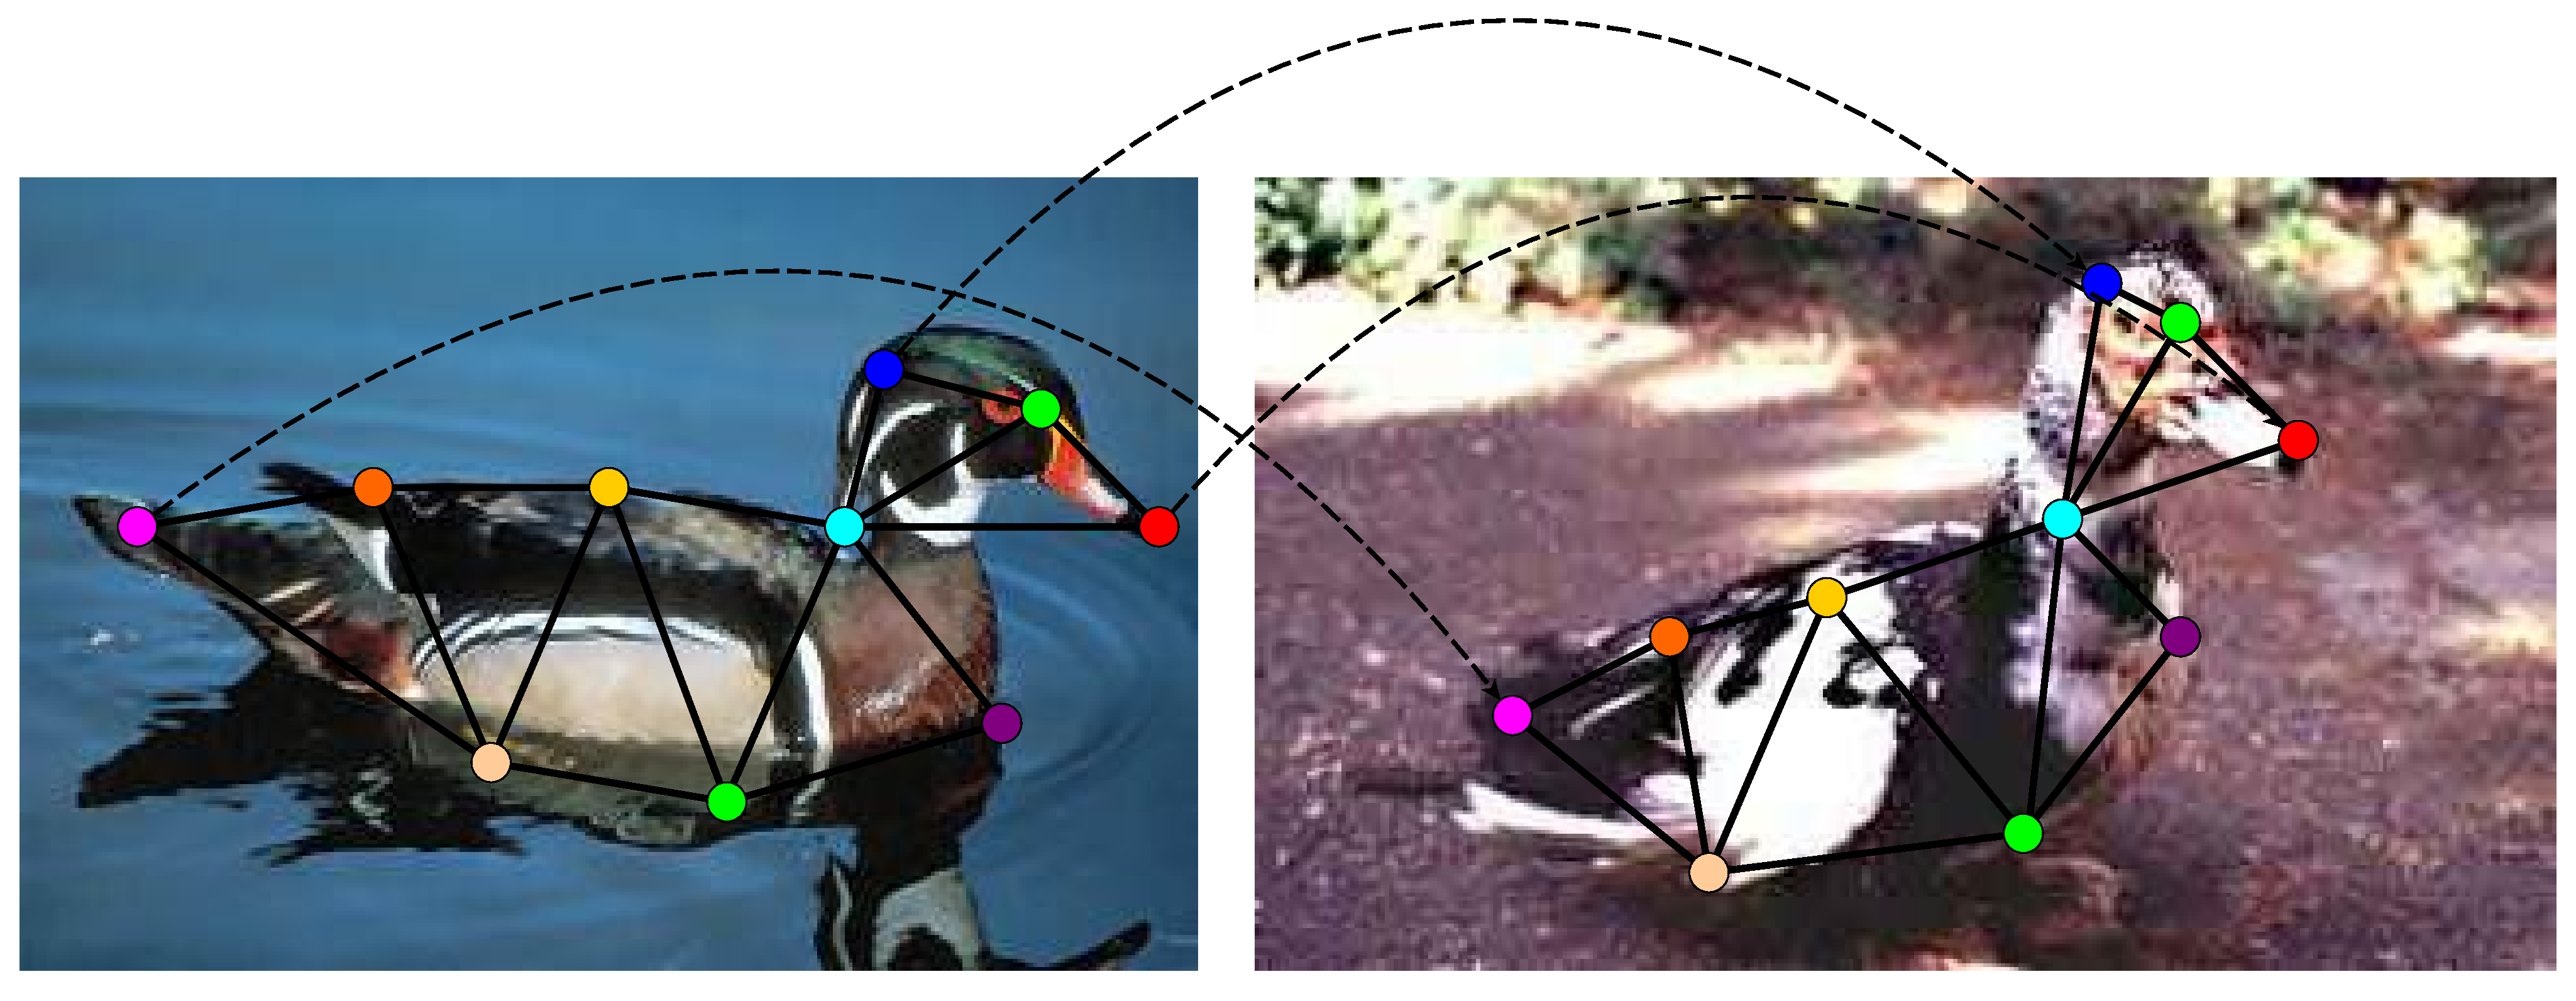
\includegraphics[width=5cm]{fig/ducks_12.pdf}
\end{figure}
\begin{itemize}
\item image matching
\item shape matching
\item object detection
\item object tracking
\item $\dots$
\end{itemize}
\end{frame}
%--------------------------------------------------------------------------%
\begin{frame}
\frametitle{Graph matching}

A matching function between $G^I$ and $G^J$ is a mapping %between the sets of nodes of two graphs:
\\
{\hspace{4cm}$m:V^I\rightarrow V^J$}

Graph matching problem between $G^I$ and $G^J$ 
\begin{equation*}
m = \argmax_{\hat{m}}S(G^I, G^J, \hat{m})
\end{equation*}


Depending on the required properties of a matching one distinguishes
\begin{itemize}
\item exact graph matching
\item inexact graph matching
\end{itemize}

\end{frame}
%--------------------------------------------------------------------------%
\subsection{Exact graph matching}
\begin{frame}[allowframebreaks]
\frametitle{Exact graph matching}
Edge preserving mapping $m$:
$\{v_i,v_{i^\prime}\}\in E^I\Rightarrow\{m(v),m(v_{i^\prime})\}\in E^J$ % for all $v_i,v_{i^\prime}\in V^I$.

\begin{minipage}[0.2\textheight]{\textwidth}
	\begin{columns}[T]
		\begin{column}{0.6\textwidth}
			\begin{itemize}
			\item mapping $m$ is bijective $\rightarrow$ graph isomorphism (GI)
			\end{itemize}
		\end{column}
		\begin{column}{0.3\textwidth}
			\begin{figure}[h!]
			    \centering
			    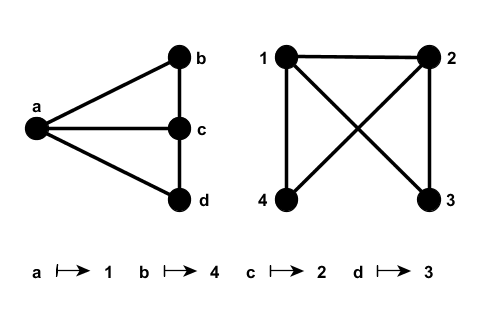
\includegraphics[width=2.3cm]{fig/GI}
			\end{figure}
		\end{column}
	\end{columns}
\end{minipage}

\begin{minipage}[0.2\textheight]{\textwidth}
	\begin{columns}[T]
		\begin{column}{0.6\textwidth}
			\begin{itemize}
			\item mapping $m$ is injective $\rightarrow$ graph monomorphism
			\end{itemize}
		\end{column}
		\begin{column}{0.3\textwidth}
			\begin{figure}[h!]
			    \centering
			    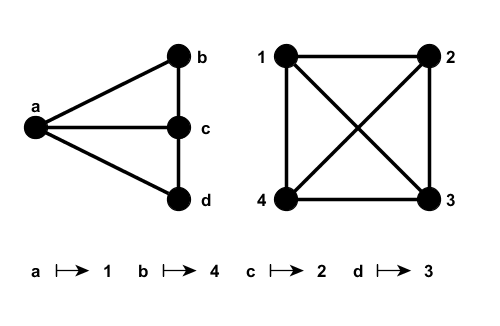
\includegraphics[width=2.3cm]{fig/monomorphism}
			\end{figure}
		\end{column}
	\end{columns}
\end{minipage}

\begin{minipage}[0.2\textheight]{\textwidth}
	\begin{columns}[T]
		\begin{column}{0.6\textwidth}
			\begin{itemize}
			\item mapping $m$ is total\hspace{15pt} $\rightarrow$ graph homomorphism
			\end{itemize}
		\end{column}
		\begin{column}{0.3\textwidth}
			\begin{figure}[h!]
			    \centering
			    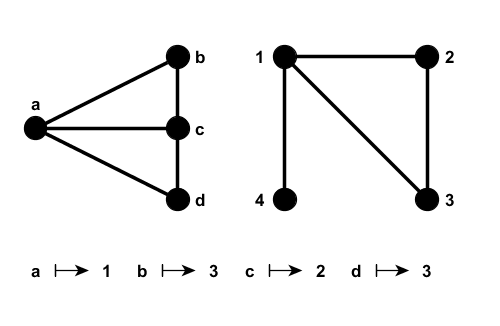
\includegraphics[width=2.3cm]{fig/homomorphism}
			\end{figure}
		\end{column}
	\end{columns}
\end{minipage}
\textcolor{red}{NP complete (except GI)~{\tiny\citep{Garey_NPComplet}}}
%\visible<2>{\textcolor{red}{NP complete(except GI)}}

\framebreak
%--------------------------------------------------------------------------%
Exact graph matching:
\begin{itemize}
\item too strict
\item cannot handle object deformation
\item time/memory consuming
\end{itemize}
\begin{figure}[htb]
	\centering
	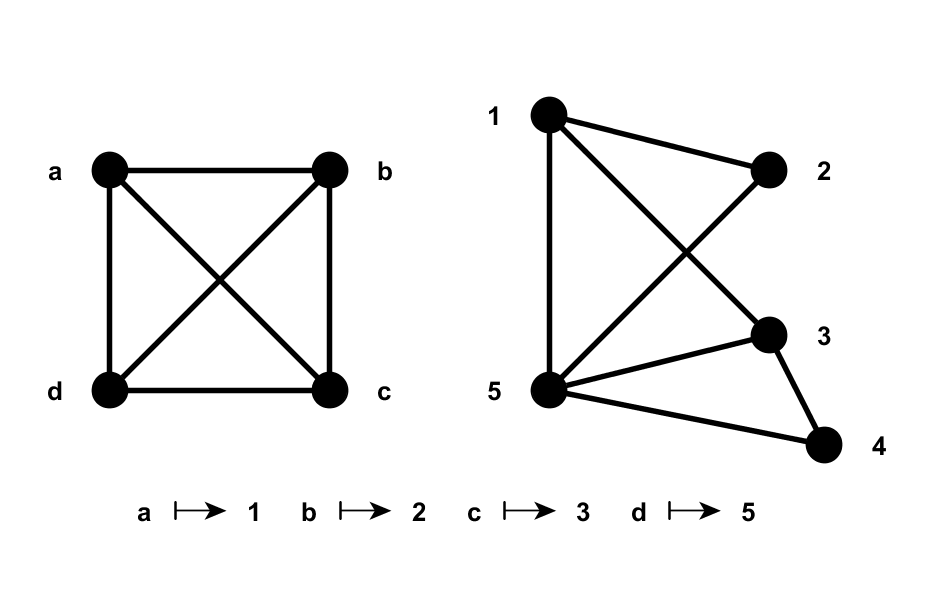
\includegraphics[width=0.5\textwidth]{fig/inexactGM}
\end{figure}
\end{frame}

%--------------------------------------------------------------------------%
\subsection{Inexact graph matching}
\begin{frame} [allowframebreaks]
\frametitle{Inexact graph matching}
Introduce similarity measure between nodes/edges in the graphs
%Do not require exact correspondences between two graphs
\begin{equation*}
m = \argmax_{\hat{m}}S(G^I, G^J, \hat{m})
\end{equation*}

\begin{equation*}
	S(G^I,G^J,m)=\sum_{\substack{m(v_i)=v_j\\m(v_i^{\prime})=v_j^{\prime}}}s_E(e_{ii^\prime},e_{jj^\prime}) + \sum_{m(v_i)=v_j}s_V(v_{i},v_{j})
\end{equation*}

\begin{itemize}
\item second-order (edge) similarity \textcolor{red}{$s_E(e_{ii^\prime},e_{jj^\prime})$}, $e_{ii^\prime}\in E^I, e_{jj^\prime}\in E^J$
\item first-order (node) similarity \textcolor{red}{$s_V(v_{i},v_{j})$}, $v_i\in V^I, v_j\in V^J$
\item assignment matrix $X\in\{0,1\}^{n_1\times n_2},\ X_{ij}=1\iff m(v_i)=v_j$, $x = \vec(X)$
\end{itemize}

\framebreak
The most common problem formulation:
\begin{block}{Quadratic Assignment Problem (NP complete)~{\tiny\citep{Burkard98thequadratic}}}
$$x^* = \arg\max \sum_{\substack{x_{ij}=1\\x_{i^\prime j^\prime}=1}}s_E(e_{ii^\prime},e_{jj^\prime}) + \sum_{x_{ij}=1}s_V(v_{i},v_{j}) $$
$$ s.t. \begin{cases}
		x\in\{0,1\}^{n_1n_2} \\
		\sum_{i=1}^{n_1}x_{ij}\le 1 \\
		\sum_{j=1}^{n_2}x_{ij}\le 1
\end{cases}$$
\end{block}
Using matrix notation : $\arg\max_{x}{x^TSx}$, $S$ is a similarity (or affinity) matrix

%Algorithms that solve this problem can be optimal or suboptimal.

\framebreak

Solution techniques~{\tiny\citep{Conte2004}}
\begin{itemize}
\item discrete optimization
	\begin{itemize}
	\item tree search~{\tiny\citep{Bunke1983_inexactGM,Shapiro1981,Fu1979,Wang1995}}
	\item simulated annealing~{\tiny\citep{Herault1990_SimulatedAnnealing}}
	\end{itemize} 
\item continuous optimization
	\begin{itemize}
		\item constraint relaxation~{\tiny\citep{Rangarajan1996_GAGM,Leordeanu2009_IPFP,FastPFP,Vogelstein_BrainGraphs,Zazlavskiy2008_PATH}}
		\item spectral methods~{\tiny\citep{Leordeanu2005_SM,Umeyam1988}}
		\item probabilistic frameworks~{\tiny\citep{Armiti2014,Hancock_Kittler,Hancock_EM_SVD,Sanrom2012}}
		\item clustering~{\tiny\citep{Hancock_ModalClusters,Cho2009_AgglClustering,Hancock_GM_SpectralPart,Lyzinski2015}}
	\end{itemize} 
\end{itemize}
\end{frame}
%--------------------------------------------------------------------------%
\begin{frame}
\frametitle{Drawback of the existing algorithms}

\begin{itemize}
\item most of the algorithms are developed for matching relatively small graphs ($\sim 150$ nodes)
\item scale badly due to the polynomial increase of time and storage demand
\item algorithms for the big graphs use another formulation of the graph matching optimization problem\\
\vspace{5pt}
{\centering
$x^* = \argmin_{X}\|A^I-XA^JX^T\|^2+\|D^I-XD^J\|^2_2$}
\end{itemize}

\end{frame}
%--------------------------------------------------------------------------%
\begin{frame}
\frametitle{Aim of the master's thesis}


\begin{itemize}
\item a novel framework that should help to extend the usability
of existing graph matching algorithms to bigger graphs
%\item iterative algorithm that allows to improve initial subdivision into subproblems
\end{itemize}
\vspace{10pt}
Idea:\\
\hspace{10pt} subdividing initial problem into a set of smaller problems, which can be easily handled with existing algorithms\\
\hspace{10pt}$\Rightarrow$ a variant of the well-known divide-and-conquer paradigm

\end{frame}
%--------------------------------------------------------------------------%
%--------------------------------------------------------------------------%
\section{Two level graph matching framework (2LevelGM)}

\begin{frame}
\frametitle{Complexity reduction}
\begin{block}{}
\tiny
$$x^* = \arg\max x^TSx $$
$$ s.t. \begin{cases}
		x\in\{0,1\}^{n_1n_2} \\
		\sum_{i=1}^{n_1}x_{ij}\le 1 \\
		\sum_{j=1}^{n_2}x_{ij}\le 1
\end{cases}$$
\end{block}

\begin{itemize}
\item set of candidate correspondences~{\tiny \citep{Cho2012_ProgressiveGM}}
\item sparse affinity matrix
\item subdivide problem into a set of smaller subproblems
\visible<2->{\hspace{10pt}\textcolor{red}{$\leftarrow$\\}}
\visible<3->{Similar works:
			\begin{itemize}
				\item semisupervised case~{\tiny\citep{Lyzinski2015}}
				\item another objective function~{\tiny\citep{Lyzinski2015,Hancock_ModalClusters,Hancock_GM_SpectralPart}}
				\item special kind of subproblem~{\tiny\citep{Hancock_GM_SpectralPart,CliqueGraph_CVPR2015}}
			\end{itemize}}
\end{itemize}
\end{frame}
%--------------------------------------------------------------------------%
\begin{frame}
\frametitle{Two level graph matching framework}
Lower level: initial graphs $G^I$, $G^J$\\
Higher level: simplified graphs (anchor graphs $A^I$, $A^J$)\\
\begin{figure} [h]
	\centering
	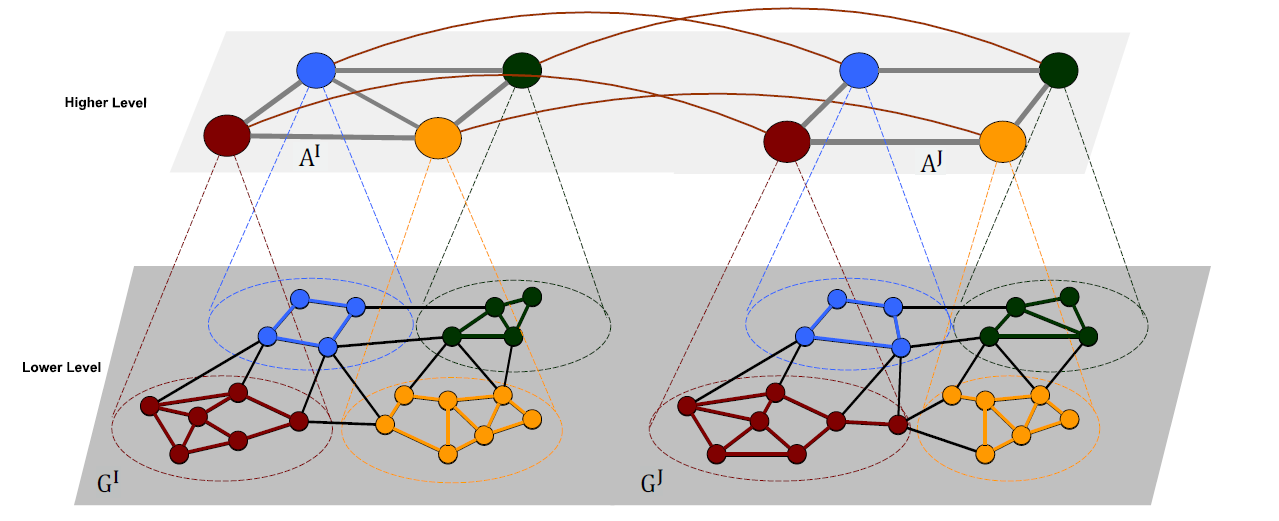
\includegraphics[scale=0.35]{fig/2levelGM/twolevels3.png}
\end{figure}
\end{frame}
%--------------------------------------------------------------------------%
\begin{frame}
\frametitle{Anchor graph construction}
Goal: $G^I=(V^I,E^I, D^I)\rightarrow A^I=(V^{Ia},E^{Ia},U^{Ia})$

Equivalent: partitioning of $G^I\supset(G^I_1\cup\dots\cup G^I_{|V^{Ia}|})$

Done by: \begin{itemize}
			\item grid with $r$ rows and $c$ columns
			\item graph coarsening algorithms: Heavy Edge Matching (HEM) and Light Edge Matching (LEM)
		\end{itemize}
\end{frame}
%--------------------------------------------------------------------------%
\begin{frame}
\frametitle{Anchor graph and subgraph matching}
Goal: find correspondences between two anchor graphs $A^I=(V^{Ia},E^{Ia},U^{Ia})$ and $A^J=(V^{Ja},E^{Ja},U^{Ja})$

\begin{itemize}
	\item edge similarity: compare length of the edges beween anchors
	\item node similarity: 
	\begin{itemize}
		\item score of the matching of $G^I_k$ and $G^J_p$
		\item define anchor attributes based on the $D^I,D^J$ and/or on the geometry of $G^I,G^J$
	\end{itemize}
\end{itemize}

Match anchor graphs and subgraph using some existing algorithm (e.g.~RRWM~{\tiny\citep{Cho2010_RRWM}})
\end{frame}

%--------------------------------------------------------------------------%
\begin{frame}
\frametitle{Graph partition update}
\begin{enumerate}
\item estimate an affine transformation between matched subgraphs (point set registration problem)
\item let nodes "vote" to which subgraphs they should belong to
\end{enumerate}
\begin{figure} [h]
	\centering
	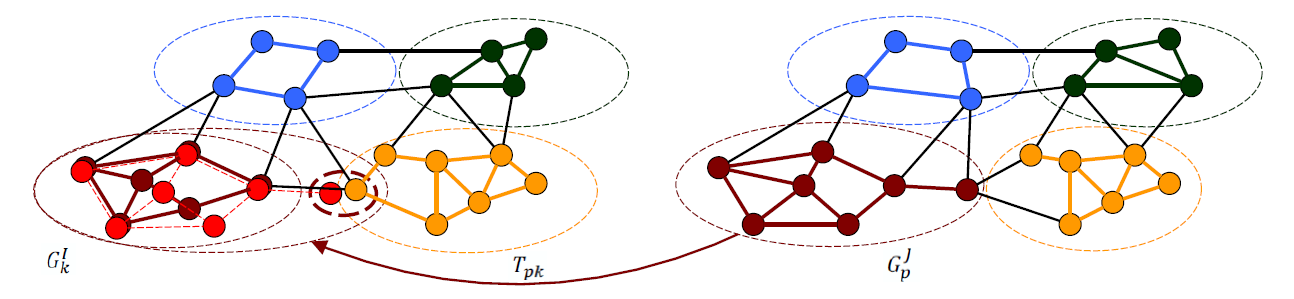
\includegraphics[scale=0.35]{fig/2levelGM/update.png}
\end{figure}
\end{frame}
%--------------------------------------------------------------------------%
%\begin{frame}
%\frametitle{Complexity}
%%complexity of a selected graph matching algorithm $\mathcal{O}(f_{GM}(n_1,n_2))$
%\begin{itemize}
%%\item Graph partitioning: $\mathcal{O}(n_2^2)$ 
%%\item Codebook of node attributes: 
%\item size of the anchor graphs and subgraphs
%\item number of iterations
%\end{itemize}
%\end{frame}
%--------------------------------------------------------------------------%
%--------------------------------------------------------------------------%
\section{Evaluation} 
\begin{frame}
\frametitle{Evaluation}
%\centering 
%{\Huge Evaluation}
Two ways of evaluation have been used
\begin{itemize}
\item synthetic data
\item real data
\end{itemize}

The quality is measured by the matching score and accuracy of an obtained solution together with the running time in seconds needed to find it.

\end{frame}

\subsection{Synthetic data}
\begin{frame}[allowframebreaks]
\frametitle{Synthetic data}
\centering
%$G^I, G^J$ are two complete graphs. $G^J$ is a copy of $G^I$ with additional outlier nodes and random shift in the node positions.

\begin{figure}
	\begin{subfigure}[b] {0.32\textwidth}
		\centering
		\includegraphics[width=2cm]{"fig/evaluation/SyntheticTest/no_descr/Results_v4.3.3/Test2/accuracy_avg10t"} 
	\end{subfigure}
	\begin{subfigure}[b] {0.32\textwidth}
		\centering
		\includegraphics[width=2cm]{"fig/evaluation/SyntheticTest/no_descr/Results_v4.3.3/Test2/score_avg10t"} 
	\end{subfigure} 
	\begin{subfigure}[b] {0.32\textwidth}
		\centering
		\includegraphics[width=2cm]{"fig/evaluation/SyntheticTest/no_descr/Results_v4.3.3/Test2/time_summary_avg10t"} 
	\end{subfigure} 
%	\caption[Performance of the 2LevelGM with non-attributed anchor graphs on synthetic data (test $1$)]{Performance of the 2LevelGM with non-attributed anchor graphs on synthetic data: test $1$ ($n_1=100$, $\bar{n}=0$, $\theta=100\%$)}
\end{figure}
\vspace{-20pt}
\begin{figure}
	\begin{subfigure}[b]{0.32\textwidth}
		\centering
		\includegraphics[width=2cm]{"fig/evaluation/SyntheticTest/no_descr/Results_v4.3.3/Test3/accuracy_avg10t"} 
	\end{subfigure}%% 
	\begin{subfigure}[b]{0.32\textwidth}
		\centering
		\includegraphics[width=2cm]{"fig/evaluation/SyntheticTest/no_descr/Results_v4.3.3/Test3/score_avg10t"} 
	\end{subfigure} 
	\begin{subfigure}[b]{0.32\textwidth}
		\centering
		\includegraphics[width=2cm]{"fig/evaluation/SyntheticTest/no_descr/Results_v4.3.3/Test3/time_summary_avg10t"} 
	\end{subfigure} 	
%	\caption[Performance of the 2LevelGM with non-attributed anchor graphs on synthetic data (test $2$)]{Performance of the 2LevelGM with non-attributed anchor graphs on synthetic data: test $2$ ($n_1=100$, $\bar{n}\in[0,50]$, $\sigma^2=0$, $\theta=100\%$)}
\end{figure}
\vspace{-20pt}
\begin{figure}
		\begin{subfigure}[b]{0.32\textwidth}
			\centering
			\includegraphics[width=2cm]{"fig/evaluation/SyntheticTest/no_descr/Results_v4.3.3/Test1/accuracy_avg10t"} 
		\end{subfigure}%% 
		\begin{subfigure}[b]{0.32\textwidth}
			\centering
			\includegraphics[width=2cm]{"fig/evaluation/SyntheticTest/no_descr/Results_v4.3.3/Test1/score_avg10t"} 
		\end{subfigure} 
		\begin{subfigure}[b]{0.32\textwidth}
			\centering
			\includegraphics[width=2cm]{"fig/evaluation/SyntheticTest/no_descr/Results_v4.3.3/Test1/time_summary_avg10t"} 
		\end{subfigure} 	
%	\caption[Performance of the 2LevelGM with non-attributed anchor graphs on synthetic data (test $3$)]{Performance of the 2LevelGM with non-attributed anchor graphs on synthetic data: test $3$ ($n_1=100$, $\bar{n}\in[0,50]$, $\sigma^2=0.03$, $\theta=100\%$)}
\end{figure}
\vspace{-20pt}
\begin{figure}
		\begin{subfigure}[b]{0.32\textwidth}
			\centering
			\includegraphics[width=2cm]{"fig/evaluation/SyntheticTest/no_descr/Results_v4.3.3/Test4/accuracy_avg10t"} 
		\end{subfigure}%% 
		\begin{subfigure}[b]{0.32\textwidth}
			\centering
			\includegraphics[width=2cm]{"fig/evaluation/SyntheticTest/no_descr/Results_v4.3.3/Test4/score_avg10t"} 
		\end{subfigure} 
		\begin{subfigure}[b]{0.32\textwidth}
			\centering
			\includegraphics[width=2cm]{"fig/evaluation/SyntheticTest/no_descr/Results_v4.3.3/Test4/time_summary_avg10t"} 
		\end{subfigure} 	
%	\caption[Performance of the 2LevelGM with non-attributed anchor graphs on synthetic data (test $4$)]{Performance of the 2LevelGM with non-attributed anchor graphs on synthetic data: test $4$ ($n_1=n_2=100$, $\sigma^2=0$)}
\end{figure}

Performance of the 2LevelGM with non-attributed anchor graphs

\framebreak


\begin{figure}[h]
	\begin{subfigure}[b]{0.32\textwidth}
		\centering
		\includegraphics[width=2cm]{"fig/evaluation/SyntheticTest/descr/Results_v4.3.3/Test2/accuracy_avg10t"} 
	\end{subfigure}
	\begin{subfigure}[b]{0.32\textwidth}
		\centering
		\includegraphics[width=2cm]{"fig/evaluation/SyntheticTest/descr/Results_v4.3.3/Test2/score_avg10t"} 
	\end{subfigure} 
	\begin{subfigure}[b]{0.32\textwidth}
		\centering
		\includegraphics[width=2cm]{"fig/evaluation/SyntheticTest/descr/Results_v4.3.3/Test2/time_summary_avg10t"} 
	\end{subfigure} 
%	\caption[Performance of the 2LevelGM with attributed anchor graphs on synthetic data (test $1$)]{Performance of the 2LevelGM with attributed anchor graphs on synthetic data: test $1$ ($n_1=100$, $\bar{n}=0$, $\sigma^2=0$)}
\end{figure}
\vspace{-20pt}
\begin{figure}[h]
	\begin{subfigure}[b]{0.32\textwidth}
		\centering
		\includegraphics[width=2cm]{"fig/evaluation/SyntheticTest/descr/Results_v4.3.3/Test3/accuracy_avg10t"} 
	\end{subfigure}%% 
	\begin{subfigure}[b]{0.32\textwidth}
		\centering
		\includegraphics[width=2cm]{"fig/evaluation/SyntheticTest/descr/Results_v4.3.3/Test3/score_avg10t"} 
	\end{subfigure} 
	\begin{subfigure}[b]{0.32\textwidth}
		\centering
		\includegraphics[width=2cm]{"fig/evaluation/SyntheticTest/descr/Results_v4.3.3/Test3/time_summary_avg10t"} 
	\end{subfigure} 	
%	\caption[Performance of the 2LevelGM with attributed anchor graphs on synthetic data (test $2$)]{Performance of the 2LevelGM with attributed anchor graphs on synthetic data: test $2$ ($n_1=100$, $\bar{n}\in[0,50]$, $\sigma^2=0$, $\theta=100\%$)}
\end{figure}
\vspace{-20pt}
\begin{figure}[h]
		\begin{subfigure}[b]{0.32\textwidth}
			\centering
			\includegraphics[width=2cm]{"fig/evaluation/SyntheticTest/descr/Results_v4.3.3/Test1/accuracy_avg10t"} 
		\end{subfigure}%% 
		\begin{subfigure}[b]{0.32\textwidth}
			\centering
			\includegraphics[width=2cm]{"fig/evaluation/SyntheticTest/descr/Results_v4.3.3/Test1/score_avg10t"} 
		\end{subfigure} 
		\begin{subfigure}[b]{0.32\textwidth}
			\centering
			\includegraphics[width=2cm]{"fig/evaluation/SyntheticTest/descr/Results_v4.3.3/Test1/time_summary_avg10t"} 
		\end{subfigure} 	
%	\caption[Performance of the 2LevelGM with attributed anchor graphs on synthetic data (test $3$)]{Performance of the 2LevelGM with attributed anchor graphs on synthetic data: test $3$ ($n_1=100$, $\bar{n}\in[0,50]$, $\sigma^2=0.03$, $\theta=100\%$)}
\end{figure}
\vspace{-20pt}
\begin{figure}[h]
		\begin{subfigure}[b]{0.32\textwidth}
			\centering
			\includegraphics[width=2cm]{"fig/evaluation/SyntheticTest/descr/Results_v4.3.3/Test4/accuracy_avg10t"} 
		\end{subfigure}%% 
		\begin{subfigure}[b]{0.32\textwidth}
			\centering
			\includegraphics[width=2cm]{"fig/evaluation/SyntheticTest/descr/Results_v4.3.3/Test4/score_avg10t"} 
		\end{subfigure} 
		\begin{subfigure}[b]{0.32\textwidth}
			\centering
			\includegraphics[width=2cm]{"fig/evaluation/SyntheticTest/descr/Results_v4.3.3/Test4/time_summary_avg10t"} 
		\end{subfigure} 	
%	\caption[Performance of the 2LevelGM with attributed anchor graphs on synthetic data (test $4$)]{Performance of the 2LevelGM with attributed anchor graphs on synthetic 
\end{figure}
Performance of the 2LevelGM with attributed anchor graphs
\framebreak
\vspace{-20pt}
\begin{figure}[h] 
		\begin{subfigure}[b]{0.32\textwidth}
			\centering
			\includegraphics[width=2.0cm]{"fig/evaluation/SyntheticTest_BigGraphs/descr/Results_v4.3.3/Test1/accuracy_avg1t"} 
		\end{subfigure}
		\begin{subfigure}[b]{0.32\textwidth}
			\centering
			\includegraphics[width=2.0cm]{"fig/evaluation/SyntheticTest_BigGraphs/descr/Results_v4.3.3/Test1/score_avg1t"} 
		\end{subfigure} 
		\begin{subfigure}[b]{0.32\textwidth}
			\centering
			\includegraphics[width=2.0cm]{"fig/evaluation/SyntheticTest_BigGraphs/descr/Results_v4.3.3/Test1/time_summary_avg1t"} 
		\end{subfigure} 	\vspace{-10pt}
	\caption*{\tiny graph isomorphism}
\end{figure}
\vspace{-20pt}
\begin{figure}[h] 
		\begin{subfigure}[b]{0.32\textwidth}
			\centering
			\includegraphics[width=2.0cm]{"fig/evaluation/SyntheticTest_BigGraphs/descr/Results_v4.3.3/Test2/accuracy_avg1t"} 
		\end{subfigure}
		\begin{subfigure}[b]{0.32\textwidth}
			\centering
			\includegraphics[width=2.0cm]{"fig/evaluation/SyntheticTest_BigGraphs/descr/Results_v4.3.3/Test2/score_avg1t"} 
		\end{subfigure} 
		\begin{subfigure}[b]{0.32\textwidth}
			\centering
			\includegraphics[width=2.0cm]{"fig/evaluation/SyntheticTest_BigGraphs/descr/Results_v4.3.3/Test2/time_summary_avg1t"} 
		\end{subfigure} 	\vspace{-10pt}
	\caption*{\tiny deformation noise $\sim\mathcal{N}(0, 0.03)$}
\end{figure}
\vspace{-20pt}
\begin{figure}[h] 
		\begin{subfigure}[b]{0.32\textwidth}
			\centering
			\includegraphics[width=2.0cm]{"fig/evaluation/SyntheticTest_BigGraphs/descr/Results_v4.3.3/Test3/accuracy_avg1t"} 
		\end{subfigure}
		\begin{subfigure}[b]{0.32\textwidth}
			\centering
			\includegraphics[width=2.0cm]{"fig/evaluation/SyntheticTest_BigGraphs/descr/Results_v4.3.3/Test3/score_avg1t"} 
		\end{subfigure} 
		\begin{subfigure}[b]{0.32\textwidth}
			\centering
			\includegraphics[width=2.0cm]{"fig/evaluation/SyntheticTest_BigGraphs/descr/Results_v4.3.3/Test3/time_summary_avg1t"} 
		\end{subfigure} 	\vspace{-10pt}
	\caption*{\tiny omit $90\%$ of edges}
\end{figure}
Comparison of 2LevelGM, GLAG and PATH on bigger graphs
\end{frame}
%--------------------------------------------------------------------------%
\subsection{Real data}
\begin{frame}[allowframebreaks]
\frametitle{Image affine transformation}

\begin{figure}[h] 
		\begin{subfigure}[b]{0.32\textwidth}
			\centering
			\includegraphics[width=2cm]{"fig/evaluation/ImageTrafo/Img_pair1"} 
		\end{subfigure}
		\begin{subfigure}[b]{0.32\textwidth}
			\centering
			\includegraphics[width=2cm]{"fig/evaluation/ImageTrafo/Img_pair2"} 
		\end{subfigure} 
		\begin{subfigure}[b]{0.32\textwidth}
			\centering
			\includegraphics[width=2cm]{"fig/evaluation/ImageTrafo/Img_pair3"}
		\end{subfigure} 	
		\begin{subfigure}[b]{0.45\textwidth}
			\centering
			\includegraphics[width=2cm]{"fig/evaluation/ImageTrafo/Img_pair4"} 
		\end{subfigure} 
		\begin{subfigure}[b]{0.45\textwidth}
			\centering
			\includegraphics[width=2cm]{"fig/evaluation/ImageTrafo/Img_pair5"}
		\end{subfigure} 	
\end{figure}

\begin{figure}[h] \centering
		\begin{subfigure}[b]{0.32\textwidth}
			\centering
			\includegraphics[scale=0.15]{"fig/evaluation/ImageTrafo/anchor_descr/using_cpd_afftrafo/performance/accuracy1"} 
		\end{subfigure} 
		\begin{subfigure}[b]{0.32\textwidth}
			\centering
			\includegraphics[scale=0.15]{"fig/evaluation/ImageTrafo/anchor_descr/using_cpd_afftrafo/performance/score1"} 
		\end{subfigure}
		\begin{subfigure}[b]{0.32\textwidth}
			\centering
			\includegraphics[scale=0.15]{"fig/evaluation/ImageTrafo/anchor_descr/using_cpd_afftrafo/performance/time1"}
		\end{subfigure}
		\caption*{Evaluation of 2LevelGM on the synthetic image dataset}
\end{figure}

\framebreak

\begin{figure} 
	\begin{center}
		\begin{subfigure}[t]{0.32\textwidth}
			\includegraphics[width=4cm]{"fig/evaluation/ImageTrafo/sIterations/It1"} 
			\caption{\scriptsize Iteration $1$}
		\end{subfigure}
		\begin{subfigure}[t]{0.32\textwidth}
			\includegraphics[width=4cm]{"fig/evaluation/ImageTrafo/sIterations/It2"} 
			\caption{\scriptsize Iteration $2$}
		\end{subfigure} 
		\begin{subfigure}[t]{0.32\textwidth}
			\includegraphics[width=4cm]{"fig/evaluation/ImageTrafo/sIterations/It3"}
			\caption{\scriptsize Iteration $3$}
		\end{subfigure} 	
		\begin{subfigure}[t]{0.32\textwidth}
			\includegraphics[width=4cm]{"fig/evaluation/ImageTrafo/sIterations/accuracy"}
			\caption{\scriptsize Accuracy\hspace{5pt}}
		\end{subfigure} 
		\begin{subfigure}[t]{0.32\textwidth}
			\includegraphics[width=4cm]{"fig/evaluation/ImageTrafo/sIterations/score"}
			\caption{\scriptsize Matching score\hspace{5pt}}
		\end{subfigure}
		\begin{subfigure}[t]{0.32\textwidth}
			\includegraphics[width=4cm]{"fig/evaluation/ImageTrafo/sIterations/gap"}
			\caption{\scriptsize Gap between current and optimal solutions}
		\end{subfigure} 	
	\end{center}		
%	\caption[Result of applying 2LevelGM to the image pair~\ref{fig:ImageTrafo_initGraphs_a}]{Result of applying 2LevelGM to the image pair~\ref{fig:ImageTrafo_initGraphs_a}. Nodes of the matched subgraphs have the same color.}
\end{figure}
\end{frame}
%--------------------------------------------------------------------------%
\begin{frame} %[allowframebreaks]
\frametitle{House data set}

\begin{minipage}[0.2\textheight]{\textwidth}
	\begin{columns}[T]
		\begin{column}{0.7\textwidth}

			\begin{figure}[h] \centering
					\begin{subfigure}[b]{0.32\textwidth}
						\centering
						\includegraphics[scale=0.12]{"fig/evaluation/HouseSeq2/anchor_descr/using_cpd_afftrafo/solution2/performance/accuracy"} 
					\end{subfigure} 
					\begin{subfigure}[b]{0.32\textwidth}
						\centering
						\includegraphics[scale=0.12]{"fig/evaluation/HouseSeq2/anchor_descr/using_cpd_afftrafo/solution2/performance/score"} 
					\end{subfigure}
					\begin{subfigure}[b]{0.32\textwidth}
						\centering
						\includegraphics[scale=0.12]{"fig/evaluation/HouseSeq2/anchor_descr/using_cpd_afftrafo/solution2/performance/time_summary"}
					\end{subfigure} 	
				\caption*{Evaluation of 2LevelGM on the CMU House sequence: not extrapolated solution}
			\end{figure}
			\vspace{-20pt}
			\begin{figure}[h] \centering
					\begin{subfigure}[b]{0.32\textwidth}
						\centering
						\includegraphics[scale=0.12]{"fig/evaluation/HouseSeq2/anchor_descr/using_cpd_afftrafo/ext_solution2/performance/accuracy"} 
					\end{subfigure} 
					\begin{subfigure}[b]{0.32\textwidth}
						\centering
						\includegraphics[scale=0.12]{"fig/evaluation/HouseSeq2/anchor_descr/using_cpd_afftrafo/ext_solution2/performance/score"} 
					\end{subfigure}
					\begin{subfigure}[b]{0.32\textwidth}
						\centering
						\includegraphics[scale=0.12]{"fig/evaluation/HouseSeq2/anchor_descr/using_cpd_afftrafo/ext_solution2/performance/time_summary"}
					\end{subfigure} 	
				\caption*{Evaluation of 2LevelGM on the CMU House sequence: extrapolated solution}
			\end{figure}

		\end{column}
		
		\begin{column}{0.3\textwidth}
			\begin{figure}[h!]
				\begin{subfigure}[b]{0.6\textwidth}
					\centering
					\includegraphics[width=2cm]{"fig/evaluation/HouseSeq2/anchor_descr/using_cpd_afftrafo/solution/fi_1_ProgGM"} 
					\caption{\tiny accuracy $11.63\%$}
				\end{subfigure}\\
				\begin{subfigure}[b]{0.6\textwidth}
					\centering
					\includegraphics[width=2cm]{"fig/evaluation/HouseSeq2/anchor_descr/using_cpd_afftrafo/ext_solution/fi_1_ProgGM"} 
					\caption{\tiny accuracy $100\%$}
				\end{subfigure}
			\end{figure}
		\end{column}
	\end{columns}
\end{minipage}
\end{frame}
%--------------------------------------------------------------------------%
%--------------------------------------------------------------------------%
\section{Conclusions}
\begin{frame} %[allowframebreaks]
\frametitle{Conclusions}
	The developed algorithm
	\begin{itemize}
		\item solves inexact graph matching problem
		\item is fast
		\item allows application of existing algorithms to bigger graphs
		\item shows very good results for (sub)graph isomorphism problems
		\item handles reasonably the affine deformations in graph structure
	\end{itemize}

	It has following properties:
	\begin{itemize}
		\item it is sensible to non-affine deformations in graph structure
%		\item  with non-affine transformations
		\item it's complexity depends on the number of iterations and on the size of the anchor graphs and subgraphs
		\item anchor attributes for anchor graph matching are preferred
	\end{itemize}
\end{frame}

%--------------------------------------------------------------------------%
\begin{frame} %[allowframebreaks]
\frametitle{Future work}
	\begin{itemize}
		\item more sophisticated graph partitioning techniques
		\item improvement of anchor attributes
		\item further improvement of the update rule
		\item probabilistic matching framework
		\item hierarchical method
	\end{itemize}
\end{frame}
%--------------------------------------------------------------------------%
%--------------------------------------------------------------------------%
\begin{frame}{The end}
\centering
\LARGE
\color{red}
Thank you for your attention!
%\nocite{Kleinberg}
%\nocite{ZheZhao2}
%\nocite{CIS}
%\nocite{HITS_Lecture4_Cornell}
%\nocite{BeamerTheme} 
\nocite{Cho_LearningG}
\end{frame}
%--------------------------------------------------------------------------%
\begin{frame}
\centering
\begin{figure}
	\includegraphics{who.png}
\end{figure}
\end{frame}
%--------------------------------------------------------------------------%
\begin{frame}[allowframebreaks]
	\frametitle{References}
	\bibliographystyle{plainnat}
	\bibliography{bibliographie}
\end{frame} 

\end{document}
%--------------------------------------------------------------------------%
%--------------------------------------------------------------------------%
%--------------------------------------------------------------------------%
